\section{Circuiti}
\begin{figure}[width=0.7\textwidth]
 \centering 
 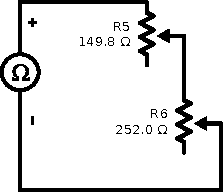
\includegraphics{Eletr1ResSerie.pdf} 
 \caption{Resistenza in serie} 
 \label{gr:02_graph_4.tex}
\end{figure}

\begin{figure}[width=0.7\textwidth]
 \centering 
 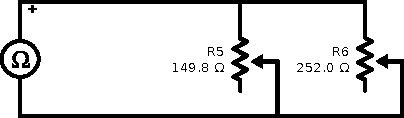
\includegraphics{Eletr1respar.pdf} 
 \caption{Resistenza in parallelo} 
 \label{gr:02_graph_4.tex}
\end{figure}

\begin{figure}[width=0.7\textwidth]
 \centering 
 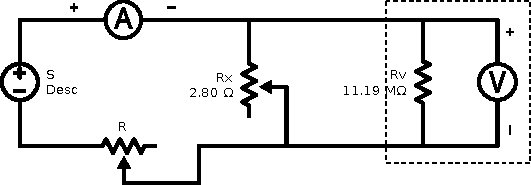
\includegraphics{Eletr1VoltAmpere.pdf} 
 \caption{Misura voltamperometrica} 
 \label{gr:02_graph_4.tex}
\end{figure}

% \begin{figure}[width=0.7\textwidth]
%  \centering 
%  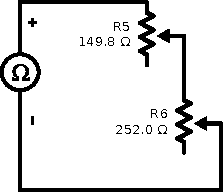
\includegraphics{Eletr1_ResSerie.pdf} 
%  \caption{Eletr1_ResSerie.pdf} 
%  \label{gr:02_graph_4.tex}
% \end{figure}

\begin{figure}[width=0.7\textwidth]
 \centering 
 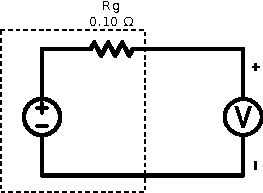
\includegraphics{Eletr1ResGeneratore.pdf} 
 \caption{Resistenza del generatore (I)} 
 \label{gr:02_graph_4.tex}
\end{figure}

\begin{figure}[width=0.7\textwidth]
 \centering 
 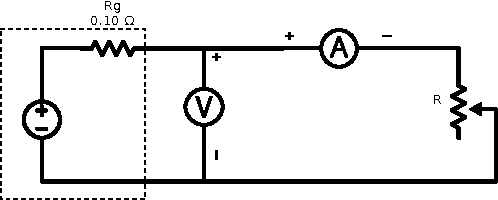
\includegraphics{Eletr1ResGeneratore2.pdf} 
 \caption{Resistenza del generatore (II)} 
 \label{gr:02_graph_4.tex}
\end{figure}

\begin{figure}[width=0.7\textwidth]
 \centering 
 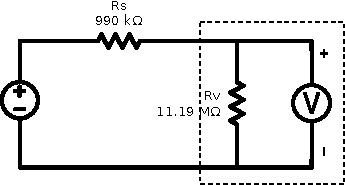
\includegraphics{Eletr1ResVoltmetro.pdf} 
 \caption{Resistenza voltmetro} 
 \label{gr:02_graph_4.tex}
\end{figure}

\begin{figure}[width=0.7\textwidth]
 \centering 
 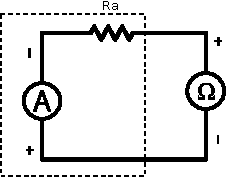
\includegraphics{Eletr1ResAmperometro.pdf} 
 \caption{Resistenza amperometro} 
 \label{gr:02_graph_4.tex}
\end{figure}